
\documentclass{cimenics}
%\input psfig.sty

%\renewcommand\figurename{Figura}
%\renewcommand\tablename{Tabla}
%\renewcommand\refname{REFERENCIAS}
%%\usepackage[ansinew]{inputenc}
%%\usepackage{pstricks}
%%\usepackage{graphicx}
%\usepackage[plainpages=false,pdfpagemode={FullScreen},bookmarksopen,bookmarksnumbered,colorlinks]{hyperref} %original way
%%\usepackage[plainpages=false,bookmarksopen,bookmarksnumbered,colorlinks]{hyperref}

%\renewcommand\figurename{Figura}
%\renewcommand\tablename{Tabla}
%\renewcommand\refname{REFERENCIAS}
\usepackage[ansinew]{inputenc}
\usepackage{pstricks}
\usepackage{graphicx}
\usepackage[plainpages=false,pdfpagemode={FullScreen},bookmarksopen,bookmarksnumbered,colorlinks]{hyperref}


\title{DIGITAL PREOPERATIVE PLANNING FOR LONG-BONE FRACTURES}

\author{Esmitt Ram\'irez J.\\Ernesto Coto}

\heading{E.Ram\'irez and E. Coto}


\address{\noindent \textit{esmitt.ramirez@ciens.ucv.ve\\ernesto.coto@ciens.ucv.ve}\\
%\textit{ernesto.coto@ciens.ucv.ve}\\
Centro de Computaci\'on Gr\'afica, Universidad Central de Venezuela. Los Chaguaramos, Caracas-Venezuela%}
\author{}

\address\noindent}

%\break BEM}

\abstract{ Nowadays, fracture management is an essential part of
everyday clinical decision-making prior to any fracture-related
surgery. The way to carry out such preoperative planning involves
tracing the bones over paper using the X-Rays, and then placing
the resulting drawings together as if reconstructing the fractured
bones. This action, although proven effective, is quite
rudimentary and time consuming. In recent years, a
significant effort has been dedicated to the building of computer systems
for aiding the preoperative planning of fracture-related
surgeries. This paper describes a new CAOS (Computer Aided
Orthopedic Surgery) system for fractures, which considerably
reduces the time required for the surgeon to plan a surgery. While
planning can often take up to 25 minutes, the described system can
reduce this time to a maximum of 5 minutes. The system also
includes a database of fracture types and a database of implants.}

\keywords{Preoperative planning, X-Ray images, Long-bone fracture,
CAOS}

\begin{document}

\section{INTRODUCTION}

Since Wilhelm R\"{o}entgen discovered the X-Rays in 1985
\cite{HOLL90}, medical imaging have evolved considerably into
techniques such as: Fluoroscopy, Ultrasound (US), Computed
Tomography (CT), Magnetic Resonance (MR), etc. All these imaging
modalities are a fundamental base to medical diagnosis in modern
healthcare systems. Currently, most imaging modalities produce
digital images. These images can be displayed and analyzed in a
medical workstation for a prompt medical diagnosis. This is the
motivation for the creation of modern CAD (Computer Aided
Diagnosis) systems.

CAD systems that give support to an orthopedic surgeon in
preoperative surgery planning for musco-skeletal system are called
CAOS. Preoperative surgery planning is an important step before an orthopedic surgery, since
it defines which procedures should be followed during surgery.
Additionally, it is an exact guide to determinate the final result
of the surgery. Preoperative planning can be done manually, although
this is often imprecise, requires many tools and it could take a
considerable amount of time. When a CAOS system is used instead,
the planning is very precise, it requires nothing additional to
the medical workstation and it can be done in a timely manner.

Nowadays, although manually planning is still performed in some
hospitals, the use of CAOS systems is rapidly spreading as more
hospitals acquire digital imaging systems \cite{GIGE00}. This
paper describes the design and development of a new CAOS system
for preoperative planning for bone fractures. The system
allows the surgeon to plan the surgery using the X-Rays images
directly, and includes a database of fracture types as
defined by the AO (\emph{Arbeitsgemeinschaft f\"ur
Osteosynthesefragen} - Association for the Study of Internal
Fixation) Foundation, and a database of plates, screws, pins and
nails from different manufacturers. It also allows interactive
plate deformation for fracture reduction. In this paper, we
describe our solution to preoperative planning for long-bone
fracture to produce an interactive and low-cost system.

The following section presents an overview on preoperative
planning for bone fractures. Section 3 describes our proposed
preoperative planning scheme for CAOS systems. Section 4 shows the
results we obtained after testing the system. Section 5 describes
conclusions and future work.

%to do later: explain sections

%%%%%%%%
%
%%%%%%%%
\section{PREOPERATIVE PLANNING FOR BONE FRACTURES}

Preoperative planning is an important step that all surgeons
should follow prior to performing any surgical procedure. The main
purpose of this planning is determining the final result of the
surgery and set up the surgical technique to apply.

As explained in \cite{STAN07}, preoperative plans for bone
fractures can be done manually tracing preoperative drawings in
paper, see Fig. \ref{fig:planificacion}\color{red}A\color{black}.
Using the trace paper it is possible to understand the complexity
of the fracture, shape of the reduction, treatment of the
biomechanical principle and choosing the correct implant to
use.

\begin{figure}[htb]
    \centering
    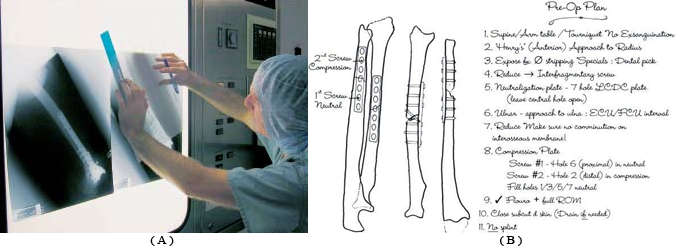
\includegraphics[width=1.0\columnwidth]{images/planificacion3.png}
    \caption{(A) Making a trace paper. (B) Illustration of preoperative plan detailing operative surgical steps, implants and equipment.}
    \label{fig:planificacion}
\end{figure}

Preoperative planning consists on creating the trace paper of
fracture segments and obtaining a surgical guide corresponding
with the area that is going to be operated. For the planning to be
performed, the following materials are necessary: fracture X-Ray
plate, paper for tracing, implant templates, goniometer, markers
and a viewbox with acceptable lighting.

To construct the plan it is important to have an X-Ray of good
quality. Place the X-Ray in the viewbox for a better contrast.
Next, draw the border of the bones using markers. Use a goniometer
to obtain different measurements for different fractured areas.
After applying this procedure it is possible to obtain different
pieces of fractures. The main idea is puzzling these pieces and
placing them on their correct position. Moreover, it is possible
to use implants for fracture reduction. These implants can be
plates, screws, pins or nails. The implants should also be
measured and taken into account in the planning. Finally, over the
trace paper, certain information must be written such as: patient
name, surgical procedure, additional tools, post-operative care,
etc. see Fig. \ref{fig:planificacion}\color{red}B \color{black}.
The selection of the surgical procedure is based on many
characteristics of the fracture or osteotomy such as: bone,
sector, trace type, number of fragments, size of fragments and
others. Before performing a surgery, a plan has to include all
sorted steps necessary for the surgery.

Although this manual procedure has proven useful, it is very time
consuming and error prone. In past years \cite{CIT07}, a
variety of support software systems to surgery in fracture
reduction has been used. These systems are called CAOS. They are the center of attention of
different research centers worldwide. With a CAOS system it is
possible appending any implant over a preoperative plan just using
a digital repository of implants. Computerized templates are now
available that allow preoperative planning to be perform directly
on digital images, eliminating the pen-and-paper method. This
situation makes the process more accurate and repeatable than the
manual technique. The following sections describe a new
preoperative planning scheme, implemented in a new CAOS system
completely developed at our research center.

%%%%%%%%
\section{PROPOSED PREOPERATIVE PLANNING SCHEME}

In our proposed planning scheme, we shown an eight-step-process:
image acquisition, calibration, segmentation and puzzling, implant
placement, implant deformation, tracing paper generation and
report generation, see Fig \ref{fig:scheme}. In a previous work \cite{RAM09}, we describes this scheme  only from a theoretical point of view. In the following subsections, we present implementation details of a CAOS system based on this scheme.

\begin{figure}[htb]
    \centering
    \includegraphics{images/schemev13.png}
    \caption{Proposed Preoperative Planning Scheme.}
    \label{fig:scheme}
\end{figure}

\subsection{Image Acquisition}

In this stage, images are captured using a digital camera or
loaded from DICOM (Digital Imaging and Communication in Medicine)
files. With the first approach, doctors can place the X-Ray over a
viewbox and take a picture to obtain a digital image. In this way,
we can use a conventional X-Ray plate. Note that image acquisition
is essential in the planning process and therefore the pictures
taken should be taken under optimal conditions (lighting, distance
to shoot, etc.). With the second approach the images can be loaded
from CR (Computer Radiography) or RG (Radiographic Imaging) DICOM
files.

\subsection{Image Calibration}

Frequently, surgeons need to take measurements for many reasons,
such as calculating the dimension of the implants for the patient,
calculating the width/height of a bone segment, etc. Generally,
these measurements are given in millimeters. Our system provides
tools to perform different kinds of measures (length, angle, etc.)
along with tools for comments and annotations. However, images
taken with digital cameras might have been taken from different
distances, providing different pixel resolutions. Assuming a fixed
pixel resolution for all images leads to huge mistakes in the
measurements. This problem should be fixed using a calibration
procedure.

Our calibration process starts opening holes in the X-Ray plates
with a two-hole paper punch, see Fig. \ref{fig:cal}\color{red}A
\color{black}.  The holes are detected automatically using
morphological operations. This requires a multipass algorithm
using a Structuring Element (SE) to search for both circles. The
size of the SE is dynamic and dependent on the region where the
circles are placed. Since the distance between the holes in the
punch is known, once the holes are detected in the image it is
possible to calculate the pixel resolution and calibrate the
images.

\begin{figure}[htb]
    \centering
    \includegraphics[width=0.75\columnwidth]{images/calibration4_copy.png}
    \caption{(A) Holes opened with paper punch allows image calibration. In this image there is a distance of 12.5 mm. between holes.
    (B) Segments with their control polygons over a long-bone fracture.}
    \label{fig:cal}
\end{figure}

\subsection{Image Enhancement}

This stage is required so as to obtain a better contrast on the
images. A manual window/level adjustment is performed at a
workstation, and the user is responsible for the quality and
enhancement of the displayed image. This stage is commonly used
for medical images enhancement.

\subsection{Fracture Segmentation and Puzzling}

%
This is a very important step in our scheme. In this stage,
surgeons can use the mouse to place the fragments produced during
fracture reduction in their anatomically correct places
(puzzling). The segmentation sub-stage can be manual or
semi-automatic. In manual mode, a surgeon marks a series of points
around fracture fragments of interest. These points define a
control polygon. A fracture may have several of them. In
semi-automatic mode, a Canny border detection algorithm is used
\cite{CANNY86}. This algorithm finds a possible border of the
fragment. The user is allowed to modify the border if necessary.
Fig. \ref{fig:cal}\color{red}B \color{black} shows an example of
this process.

In the puzzling sub-stage, each fracture segment is selected and
placed in their correct anatomical position over the bone.
Segments can be rotated and translated but not scaled. Although it
might happen that not all segments fit perfectly in their correct
position, a very close approximation is enough for planning.

\subsection{Implant Placement}

When the puzzling process is completed, the surgeon could decide
to place an implant on the patient. Our system provides a library of
implants that contains plates, screws, pins and nails from
different manufacturers. Our system also includes a complete
library of AO fracture classifications \cite{RUEDI03}. In our
system, a MySql$\texttrademark$ database is used to store implant information such
as type, size, category, etc. Each implant is represented using a
STL (stereolithography) format file generated by Autodesk
Inventor $\texttrademark$, which stores the 3D triangulated surface of the implant.

\subsection{Implant Deformation}

Once the implant is placed, the surgeon might need to bend it
to make it fit in the correct anatomical position. The bending
process is defined as a deformation applied to a metal part by
pressure along a curved path. Implants generally are made of metal
or any alloy of it. This deformation is made by the surgeon in the
operation room using a specialized groove plier over an implant.
Our system allows the digital deformation of the implant prior to
the operation, using a variation for X-Ray images of the algorithm
proposed in \cite{BIRK03}.

\subsection{Tracing Paper and Report Generation}

Once the previous stages are completed, the results are saved in a
digital tracing paper, similar to the one in Fig.
\ref{fig:planificacion}\color{red}B\color{black}. This is the
tracing paper the surgeon will use as a guide for the surgery. It
contains annotations, measurements, fragments of bones, implants
and the input X-Ray.

In the Report Generation stage, the user can print a document
reviewing the planning process. Information such as number of
implants used, surgical technique, etc. are placed in this report.
This document is intended to be printed like a report or for
storage in a database of clinical cases.
%%%%%%%%
%
%%%%%%%%
\section{RESULTS}

The time it takes for surgeons to create a preoperative planning
manually varies from 8 to 25 minutes approximately. We installed
our system in a standard PC without specialized hardware at the
Radiology Department of the HUC (University Hospital of Caracas) in
Venezuela, and instructed two experts on how to use the system.
Once the experts became familiar with the system, the planning time
varied from 2 to 5 minutes. This is a considerable reduction of
the planning time. In addition, the experts learned how to use the system in a short time with minimal training. 

\section{CONCLUSIONS AND FUTURE WORK}

We have presented a scheme for preoperative planning for fractures
that uses image-based techniques over a conventional PC. We
proposed several stages with the purpose of creating a scalable,
detailed and maintainable workflow. Each stage can be extended
with new sub-stages and functionality without affecting the rest.
The library of implants reduces the time for the surgeon to choose
the correct implant for a fracture. In addition, the possibility
of digitally bending an implant using a 3D geometry allows a
better proximation to the actual surgery. Since no special
hardware is required, it is possible to use the system even in
rural medical facilities.

Several improvements are possible. First, a better border
detection algorithm can be used. We are planning to try
algorithms based on active contours or deformable models. Second,
for the calibration process we used a paper punch because it is a
common supply in any medical healthcare center, but this might not
be the case, and therefore we are planning to provide other
calibration options. Finally, we are planning to exploit current
technology to speed up the annotation process, e.g. speaker
annotations, medical tablet PCs, etc.

\section*{\textit{Acknowledgements}}

We would like to thank Md. Carlos S\'anchez and Eng. Othman
Falc\'on for their valuable input and experience. All medical
images used during this research project were kindly provided by
the Radiology Department at HUC, Venezuela.

%\bibliographystyle{plain}
%\bibliography{books}
\begin{thebibliography}{1}

\bibitem{CIT07}
M.~Citak, T.~N. Board, Y.~Sun, V.~Look, C.~Krettek, T.~H\"{u}fner, and
  D.~Kendoff.
\newblock Reference marker stability in computer aided orthopedic surgery: A
  biomechanical study in artificial bone and cadavers.
\newblock {\em Technol. Health Care}, 15(6):407--414, 2007.

\bibitem{RAM09}
Ram\'{i}rez E.
\newblock Planificaci\'{o}n preoperatoria digital en traumatolog\'{i}a.
\newblock Technical Report 2009-7, Central University of Venezuela, Caracas,
  April 2009.

\bibitem{BIRK03}
Birkholz H. and Jack\`{e}l D.
\newblock Image warping with feature curves.
\newblock In {\em SCCG '03: Proceedings of the 19th Spring Conference on
  Computer Graphics}, pages 199--202, NY, USA, 2003. ACM.

\bibitem{CANNY86}
Canny J.
\newblock A computational approach to edge detection.
\newblock {\em IEEE Transactions on Pattern Analysis and Machine Intelligence},
  8(6):679--698, 1986.

\bibitem{STAN07}
Stannard J., Schmidt A., and Kregor P.
\newblock {\em Surgical Treatment of Orthopaedic Trauma}.
\newblock Thieme Medical Publishers, Inc., 2007.

\bibitem{HOLL90}
Hollins M.
\newblock {\em Medical physics}.
\newblock Nelson Thornes, Basingstoke, England, 1990.

\bibitem{GIGE00}
Giger M.L.
\newblock Computer-aided diagnosis in medical imaging - {A} new era in image
  interpretation.
\newblock Technical report, The College University of Chicago, Chicago, January
  2000.

\bibitem{RUEDI03}
R\"{u}edi~T. P. and William~M. M.
\newblock {\em Principios de la {AO} en el tratamiento de las Fracturas}.
\newblock Masson, Barcelona, Spain, 2003.

\end{thebibliography}


\end{document}
